\documentclass{article}
\usepackage[spanish]{babel}
\usepackage[utf8]{inputenc}
\usepackage{johd}
\title{Tema 1. Introducción a JEE}

\author{José Antonio Fajardo Naranjo \\
	\small
	\tt{fajardonaranjoja@gmail.com} \\
	\date{}
}

\begin{document}
	\maketitle
	\begin{abstract} 
		\noindent Estos apuntes pertenecen al tema 1 de la asignatura de Desarrollo Web en entorno servidor impartida en el 2ndo curso de FPGS de DAW en el IES Martín Rivero durante el curso 2023/2024  \end{abstract}
		
	\newpage{\ }
	\tableofcontents
	\newpage{\ }
	
	\thispagestyle{empty}
	
	\section{Introducción}
	
	\paragraph{}La \textbf{tecnología JEE} (Java Enterprise Edition) se presenta como una solución propuesta por Sun Microsystems para el desarrollo de aplicaciones distribuidas. Se \textbf{basa} en el lenguaje básico Java, también conocido como \textbf{JSE} (Java Standard Edition). JEE se puede considerar como una \textbf{normativa} que describe todos los elementos que constituyen e intervienen para el funcionamiento de una aplicación distribuida.
	\\
	\\
	Define:
	\begin{itemize}
		\item Cómo se deben \textbf{desarrollar} los diferentes componentes de una aplicación (servlet, páginas JSP...).
		\item Cómo se deben \textbf{comunicar} con ellos o con otras aplicaciones (JDBC, JavaMail...).
		\item Cómo deben \textbf{organizarse} estos componentes para construir una aplicación (descriptor de despliegue).
		\item Las \textbf{restricciones} que tienen que respetar los servidores encargados de albergar estas aplicaciones.
	\end{itemize}
	\paragraph{}El cumplimiento de esta normativa permite el desarrollo de servidores para las aplicaciones que respeten esta normativa, habiendo varios disponibles con rendimiento, capacidad y precio diferente.
	\\
	\\
	La \textbf{ventaja} que ofrece JEE con \textbf{relación a tecnologías propietarias} (software privativo) reside en que cabe la posibilidad de evolucionar a otro servidor con más rendimiento sin necesidad de grandes modificaciones en la aplicación.
	
	\section{Servidores Web y servidores de aplicaciones}
	
	\paragraph{}Un \textbf{servidor Web es un servidor de archivos}. Los clientes se dirigen a él mediante el \textbf{protocolo HTTP} para obtener un recurso. Cuando el servidor Web recibe la petición HTTP, extrae de la petición el recurso solicitado, lo busca en el disco y envía el recurso dentro de la respuesta HTTP para devolverlo al cliente. Esto se resume en que el \textbf{servidor Web no realiza ningún tipo de tratamiento} en el recurso antes de transmitirlo, no importando el tipo de recurso que le es solicitado.
	Este servidor se usa para recursos \textbf{estáticos}.
	
	\paragraph{}La función de un \textbf{servidor de aplicaciones} es la de \textbf{alojar el código} y \textbf{ejecutarlo} para, posteriormente, mediante el protocolo HTTP, \textbf{devolver} el resultado de la \textbf{ejecución} del código alojado de vuelta al cliente. Este servidor se utiliza para recursos \textbf{dinámicos}.
	
	\paragraph{}La \textbf{diferencia} entre el servidor Web y el de aplicaciones radica en esto, en que, mientras el \textbf{servidor Web} sólo se dedica a \textbf{enviar archivos} indistintamente según sea solicitado por el cliente, el \textbf{servidor de aplicaciones} se encarga de \textbf{ejecutarlo} en lugar del cliente devolviendo el resultado de la ejecución como texto plano.
	
	\paragraph{}La confusión viene dada porque en ocasiones el \textbf{servidor de aplicaciones} \textbf{también} toma las \textbf{funciones} de \textbf{servidor Web}. Cuando el servidor recibe una petición del \textbf{exterior}, la parte del servidor Web la \textbf{analiza}. Si la petición es de un recurso \textbf{estático}, el servidor Web cumple \textbf{su función} y se encarga de la petición, reenviando el recurso al cliente en una respuesta HTTP. Si, por el contrario, esa petición es de un recurso \textbf{dinámico}, el servidor Web la transfiere al \textbf{servidor de aplicaciones}, ejecutando este último el código correspondiente y generando la respuesta HTTP. En caso de ser necesario, el servidor de aplicaciones puede contactar con otro servidor o base de datos para la construcción de la respuesta, que se transmite al servidor Web, encargado de transmitirla al cliente de \textbf{vuelta}.
	
	\begin{figure}[H]
		\centering
		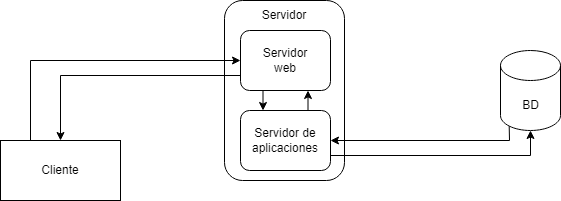
\includegraphics[scale=0.6]{images/diagramaclienteservidores1.drawio.png}
		\caption{\label{fig1}Explicación gráfica del entramado de solicitudes entre los servidores mostrado anteriormente}
	\end{figure}
	
	\paragraph{}La parte que corresponde al servidor Web en un servidor de aplicaciones suele ser peor en cuanto a rendimiento que un servidor Web dedicado. Puede esta parte ser reemplazada por uno dedicado al adjuntarle un elemento llamado redirector, que transferirá las peticiones HTTP al servidor de aplicaciones que requieran recursos dinámicos, mientras que los estáticos los gestionará el propio servidor Web y el enlace entre redirector y servidor de aplicaciones lo proporcionará un protocolo de red propietario.
	
	\begin{figure}[H]
		\centering
		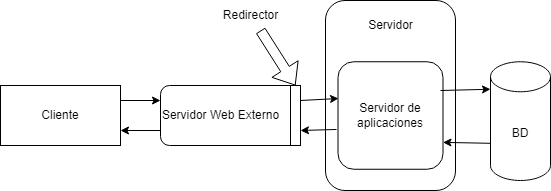
\includegraphics[scale=0.6]{images/diagramaclienteservidores2.png}
		\caption{\label{fig2}Ejemplo de solicitudes con un servidor Web dedicado}
	\end{figure}
	
	\paragraph{}Se puede optar por esta solución en caso de que el servidor de aplicaciones esté altamente solicitado. Además, este redirector puede balancear las peticiones entre varios servidores de aplicaciones que sean idénticos
	
	\begin{figure}[H]
		\centering
		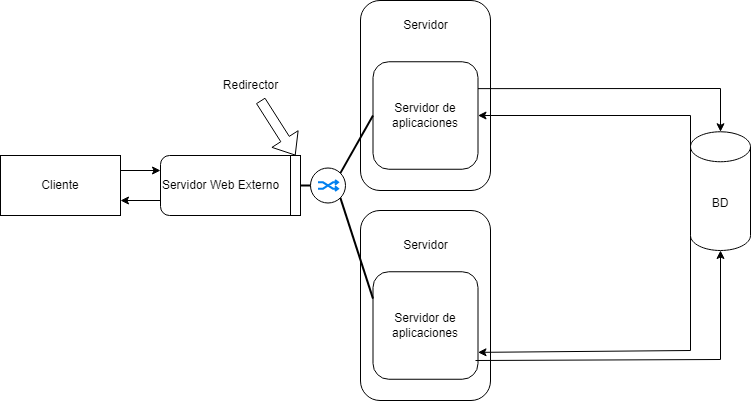
\includegraphics[scale=0.6]{images/diagramaclienteservidores3.png}
		\caption{\label{fig3}Ejemplo de solicitudes con un servidor Web dedicado y reparto de peticiones}
	\end{figure}
	
	\section{Clientes ligeros y clientes pesados}
	
	\paragraph{}Cuando se habla desde el punto de vista de las aplicaciones informáticas, se suele llamar cliente ligero a una solución que permite usar una aplicación desde un ordenador sin necesidad de instalación de ningún programa, función que realiza, por lo general, un navegador web. La mayoría de sistemas operativos llevan en su paquete este tipo de servicios. El servidor de aplicaciones se encarga del conjunto de tratamientos en este caso. La ventaja es la ausencia de intervención en los ordenadores cliente. La desventaja es la fuerte carga de solicitudes del servidor y la limitación del aspecto visual de la aplicación a las funcionalidades del lenguaje HTML, que se ayuda de otras tecnologías para mejorar la renderización gráfica de la aplicación.
	
	\paragraph{}El cliente pesado no tiene limitaciones en este ámbito. Además, permite aligerar la carga del servidor, que puede simplemente enviar al cliente los resultados en bruto de un tratamiento dejando al cliente la tarea de gestionar él mismo la presentación de estos resultados. La desventaja es el requisito de instalar la aplicación encargada del diálogo con el servidor y la presentación de los resultados en todos los ordenadores cliente. Cuando existe una nueva versión, también se ha de desplegar en todos los ordenadores cliente.
	
	\paragraph{}Pasamos por la mención de los applets, que se han quedado desactualizados.
	
	\section{Estructura de una aplicación JEE}
	
	\paragraph{}La normativa JEE describe además, cómo se debe organizar una aplicación para que pueda ser soportada por cualquier servidor de aplicaciones compatible. Una aplicación web generalmente se compone de los siguientes elementos:
	
	\begin{itemize}
		\item \textbf{Recursos estáticos}: HTML, imágenes, sonidos, CSS...
		\item \textbf{Recursos dinámicos}: servlets, JSP, Java Bean.
		\item \textbf{Librerías} de clases utilizadas por los diferentes componentes dinámicos.
		\item \textbf{Descriptor de despliegue} que permita definir los parámetros de funcionamiento de la aplicación en el servidor, los enlaces entre las URL y los recursos dinámicos de la aplicación, las páginas por defecto y de error de la aplicación, la seguridad de la misma, etc.
	\end{itemize}
	
	\begin{figure}[H]
		\centering
		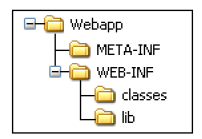
\includegraphics[scale=0.6]{images/elementosjee.png}
		\caption{\label{fig4}Árbol de organización de los elementos de una aplicación JEE}
	\end{figure}

	\paragraph{}El directorio \textbf{Webapp} del ejemplo no hace que sea obligatorio que se llame así. Algunos servidores usan el nombre de la carpeta como nombre del servidor.
	
	\paragraph{}La \textbf{carpeta META-INF} contiene el MANIFEST.MF generado por la herramienta de archivado jar. Contiene la información descriptiva del archivo cuando la aplicación es desplegada con esta forma.
	
	\paragraph{}La \textbf{carpeta WEB-INF} contiene elementos únicamente accesibles por el servidor. Se encuentra el archivo web.xml, que es el descriptor de despliegue de la aplicación.
	
	\paragraph{}El subdirectorio \textbf{classes} del directorio WEB-INF contiene el código compilado de todas las clases necesarias para el funcionamiento de la aplicación. Si las clases están definidas en paquetes, esta carpeta ha de tener un árbol con estructura idéntica a la de los paquetes de la aplicación. Estos archivos nunca se transfieren a clientes, solo el servidor instancia las clases.
	
	\paragraph{}El subdirectorio \textbf{lib} de WEB-INF contiene las librerías para el funcionamiento de la aplicación. Estas se ubican generalmente en esta carpeta en forma de archivo Java (jar). Se puede encontrar, por ejemplo, la librería que contiene un driver de acceso a una BD o librerías de etiquetas JSP personalizadas.
	
	\section{Empaquetado de una aplicación}
	
	\paragraph{}Para facilitar el despliegue de una aplicación se puede incluir todo el conjunto de archivos necesarios para el funcionamiento de la aplicación en un archivo empaquetado Java (.jar o .war). Este archivo con extensión .war se despliega automáticamente en el servidor.
	
	\paragraph{}La manipulación de un archivo empaquetado Java utilizan la sintaxis de manipulación de archivos muy similar a Unix. Estos se epaquetan internamente en formato ZIP.
	
	\subsection{Creación de un empaquetado}
	
	\paragraph{}La estructura del comando para crear un empaquetado en Java es la siguiente:
	
	\begin{centering}
		\texttt{}
	\end{centering}
	
\end{document}